\documentclass{../tudscript}

\title{Mathe VL 5}
\author{Jakob Krebs}
\begin{document}
    \sect{Stetigkeit von Funktionen}
        \ssect{Definition: reele Funktion}
            \ilmath{f: D \rightarrow \bR, D \subseteq \bR^1}
            heißt \underline{reele Funktion in einer reelen Veränderlichen}.
        \ssect{Bemerkung: Definitionsbereich}
            D ist der Definitionsbereich (die Mege der Elemente, der ein Funktionswert zugeordnet wird).
            \begin{itemize}
                \item $f(D)$ ist das Bild/Wertebereich von f
                \item $\set{(x, (f(x))) \mid x \in D}$ ist der Graph von $f$
            \end{itemize}
        \ssect{Folgendefinition der Stetigkeit}
            \ilmath{f: D \rightarrow \bR, D \subseteq \bR, a \in D}
            heißt \underline{stetig}, wenn gilt
            \ilmath{&\forall (x_n): x_n \in D \land \lim_{x \to \infty} x_n = a \\
                    &\implies \lim_{x \to \infty} f(x_n) = f(a)}
        \ssect{Bemerkung}
            \ilmath{\lim_{x \to \infty} f(x_n) = f(\lim_{x \to \infty})}
            Bei stetigen Funktionen sind die Grenzwertbestimmung und die Funktionswert
            berechnung in der Reihenfolge vertauschbar!
        \ssect{Bezeichnung}
            \ilmath{\lim_{x \to a} f(x)}
            dass heißt, für jede Folge $(x_n)$ gegen a konvergiert, konvergiert die Folge
            der Funktionswerte gegen $f(a)$.
        \ssect{Bemerkung}
            f ist stetig in a gdw,
            \begin{enumerate}
                \item $f(a)$ existiert.
                \item $\lim_{x \to a} f(x)$ existiert.
                \item $\lim_{x \to a} f(x) = f(a)$
            \end{enumerate}
            \begin{tikzpicture}
	            \draw[->] (-0.2,0) -- (4.2,0) node[right] {$x$};
	            \draw[->] (0,-0.2) -- (0,4.2) node[above] {$y$};
	            \draw[scale=1,domain=-0.2:3.9,smooth,variable=\x,blue] plot ({\x},{0.15*\x*\x+0.3*\x+0.25});
	            \node[label=below:$x_0$] at (0.5, 0) (x0) {$|$};
	            \node[label=below:$x_2$] at (1, 0) (x2) {$|$};
	            \node[label=below:$a$] at (2, 0) (a) {$|$};
	            \node[label=below:$x_3$] at (3, 0) (x3) {$|$};
	            \node[label=below:$x_1$] at (3.5, 0) (x1) {$|$};
	            \node[label=left:$f(a)$] at (0, 1.5) (fa) {$-$};
            \end{tikzpicture}
            
        \ssect{Beispiele}
            \ilmath{f(x) = \frac{x^2 -1}{x-1} = \frac{(x-1)(x+1)}{x-1}}
            Ist f(x) stetig in a = 1?
            
	    1)
            \ilmath{f(a) \text{existiert nicht}}
            also ist f(x) in a nicht stetig.

            2)
            \ilmath{\lim_{x \to 1} f(x) = \lim_{x \to 1} \frac{(x-1)(x+1)}{x-1}}
            Sei $(x_n)$ eine beliebige Folge mit $x_n \in D(f)$ und $\lim_{x \to \infty} x_n = 1$
	    \ilmath{&\lim_{x \to \infty} f(x_n) = \lim_{x \to \infty} \frac{(x-1)(x+1)}{x-1} \\
                    &= \lim_{x \to \infty} (x+1) = 1 + 1 = 2}
            D.h. GW ex. und ist 2.
            
            \begin{tikzpicture}
	            \draw[->] (-0.2,0) -- (2.2,0) node[right] {$x$};
	            \draw[->] (0,-0.2) -- (0,2.2) node[above] {$y$};
	            \draw[scale=1,domain=-0.2:1.9,smooth,variable=\x,blue] plot ({\x},{\x});
	            \node[label=below:$a$] at (1, 0) (a) {$|$};
	            \node[label=left:$f(a)$] at (0, 1) (fa) {$-$};
	            \draw[red,fill=white] (1, 1) circle (0.07);
            \end{tikzpicture}

             
        \ssect{Definition: allgemein stetig}
            \ilmath{f: D \rightarrow \bR, D \subseteq \bR}
            heißt stetig, wenn für alle $a \in D$ f stetig ist.
        \ssect{Beispiele}
            Elementare Funktionen und ihre Verknüpfungen sind auf dem gesamten
            Deinitionsbereich stetig.
            

            Der Beweis von 
            \ilmath{f: \bR \setminus 0 \rightarrow \bR: x \mapsto x^{-1}}
            stetig:
            Sei $a \in D = \bR \setminus \Set{0}$ 
            \begin{enumerate}
                \item $f(a) = \frac{1}{a}$ ex.
                \item \ilmath{\lim_{x \to \infty} f(x) = \lim_{x \to a} \frac{1}{x}}
                        Sei $(x_n)$ eine reele Folge mit $(x_n) \in D$ mit 
                        \ilmath{\lim_{x \to \infty} x_n = a}
                        \ilmath{\lim_{x \to \infty} f(x_n) = \lim_{x \to \infty} \frac{1}{x} = \frac{1}{a} \in \bR \text{ ex.}}
                \item Grenzwert ist Funktionswert
            \end{enumerate}
        	\begin{tikzpicture}
	        	\draw[->] (-2.2,0) -- (2.2,0) node[right] {$x$};
	        	\draw[->] (0,-2.2) -- (0,2.2) node[above] {$y$};
	        	\draw[scale=1,domain=-2:-0.5,smooth,variable=\x,blue] plot ({\x},{1/\x});
	        	\draw[scale=1,domain=0.5:2,smooth,variable=\x,blue] plot ({\x},{1/\x});
        	\end{tikzpicture}
        
        \ssect{Rechenregeln für stetige Funktionen}
            \ilmath{\lim_{x \to \infty} f(x) \underset{\div}{\overset{\cdot}{\pm}} g(x) = \lim_{x \to \infty} f(x) \underset{\div}{\overset{\cdot}{\pm}} \lim_{x \to \infty} g(x) }
            wobei $g(x) \neq 0$

            \ilmath{\lim_{x \to \infty} (f(x_n) \underset{\div}{\overset{\cdot}{\pm}} g(x_n)) = \lim_{x \to \infty} f(x_n)  \underset{\div}{\overset{\cdot}{\pm}} \lim_{x \to \infty} g(x_n)}


        \ssect{Satz}
	    \ilmath{f: D \rightarrow \bR, D \subseteq \bR \text{ mit } a \in D}
            stetig
            \ilmath{\iff \forall \epsilon < 0: \exists \gamma > 0: |x-a| < \gamma \implies |f(x) - f(a)| < \epsilon}
            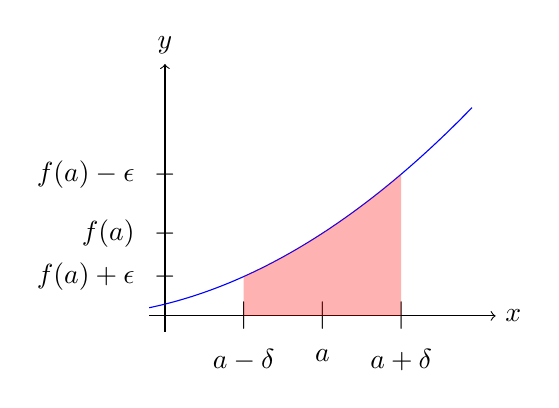
\begin{tikzpicture}
	            \draw[->] (-0.2,0) -- (4.2,0) node[right] {$x$};
	            \draw[->] (0,-0.2) -- (0,3.2) node[above] {$y$};
	            \draw[scale=1,domain=-0.2:3.9,smooth,variable=\x,blue] plot ({\x},{0.1*\x*\x+0.25*\x+0.15});
	            \node[label=below:$a-\delta$] at (1, 0) (ld) {$|$};
	            \node[label=below:$a$] at (2, 0) (a) {$|$};
	            \node[label=below:$a+\delta$] at (3, 0) (rd) {$|$};
	            \node[label=left:$f(a)+\epsilon$] at (0, 0.5) (ud) {$-$};
	            \node[label=left:$f(a)$] at (0, 1.05) (fa) {$-$};
	            \node[label=left:$f(a)-\epsilon$] at (0, 1.8) (ld) {$-$};
	            \fill [red, opacity=0.3, domain=1:3, variable=\x]
		            (1, 0)
		            -- plot ({\x},{0.1*\x*\x+0.25*\x+0.15})
		            -- (3, 0)
		            -- cycle;
            \end{tikzpicture}
\end{document}
